\PassOptionsToPackage{unicode=true}{hyperref} % options for packages loaded elsewhere
\PassOptionsToPackage{hyphens}{url}
%
\documentclass[]{article}
\usepackage{lmodern}
\usepackage{amssymb,amsmath}
\usepackage{ifxetex,ifluatex}
\usepackage{fixltx2e} % provides \textsubscript
\ifnum 0\ifxetex 1\fi\ifluatex 1\fi=0 % if pdftex
  \usepackage[T1]{fontenc}
  \usepackage[utf8]{inputenc}
  \usepackage{textcomp} % provides euro and other symbols
\else % if luatex or xelatex
  \usepackage{unicode-math}
  \defaultfontfeatures{Ligatures=TeX,Scale=MatchLowercase}
\fi
% use upquote if available, for straight quotes in verbatim environments
\IfFileExists{upquote.sty}{\usepackage{upquote}}{}
% use microtype if available
\IfFileExists{microtype.sty}{%
\usepackage[]{microtype}
\UseMicrotypeSet[protrusion]{basicmath} % disable protrusion for tt fonts
}{}
\IfFileExists{parskip.sty}{%
\usepackage{parskip}
}{% else
\setlength{\parindent}{0pt}
\setlength{\parskip}{6pt plus 2pt minus 1pt}
}
\usepackage{hyperref}
\hypersetup{
            pdftitle={Model Specification and Hyper Parameter Tuning},
            pdfauthor={Sabbir Ahmed Hemo},
            pdfborder={0 0 0},
            breaklinks=true}
\urlstyle{same}  % don't use monospace font for urls
\usepackage[margin=1in]{geometry}
\usepackage{color}
\usepackage{fancyvrb}
\newcommand{\VerbBar}{|}
\newcommand{\VERB}{\Verb[commandchars=\\\{\}]}
\DefineVerbatimEnvironment{Highlighting}{Verbatim}{commandchars=\\\{\}}
% Add ',fontsize=\small' for more characters per line
\usepackage{framed}
\definecolor{shadecolor}{RGB}{248,248,248}
\newenvironment{Shaded}{\begin{snugshade}}{\end{snugshade}}
\newcommand{\AlertTok}[1]{\textcolor[rgb]{0.94,0.16,0.16}{#1}}
\newcommand{\AnnotationTok}[1]{\textcolor[rgb]{0.56,0.35,0.01}{\textbf{\textit{#1}}}}
\newcommand{\AttributeTok}[1]{\textcolor[rgb]{0.77,0.63,0.00}{#1}}
\newcommand{\BaseNTok}[1]{\textcolor[rgb]{0.00,0.00,0.81}{#1}}
\newcommand{\BuiltInTok}[1]{#1}
\newcommand{\CharTok}[1]{\textcolor[rgb]{0.31,0.60,0.02}{#1}}
\newcommand{\CommentTok}[1]{\textcolor[rgb]{0.56,0.35,0.01}{\textit{#1}}}
\newcommand{\CommentVarTok}[1]{\textcolor[rgb]{0.56,0.35,0.01}{\textbf{\textit{#1}}}}
\newcommand{\ConstantTok}[1]{\textcolor[rgb]{0.00,0.00,0.00}{#1}}
\newcommand{\ControlFlowTok}[1]{\textcolor[rgb]{0.13,0.29,0.53}{\textbf{#1}}}
\newcommand{\DataTypeTok}[1]{\textcolor[rgb]{0.13,0.29,0.53}{#1}}
\newcommand{\DecValTok}[1]{\textcolor[rgb]{0.00,0.00,0.81}{#1}}
\newcommand{\DocumentationTok}[1]{\textcolor[rgb]{0.56,0.35,0.01}{\textbf{\textit{#1}}}}
\newcommand{\ErrorTok}[1]{\textcolor[rgb]{0.64,0.00,0.00}{\textbf{#1}}}
\newcommand{\ExtensionTok}[1]{#1}
\newcommand{\FloatTok}[1]{\textcolor[rgb]{0.00,0.00,0.81}{#1}}
\newcommand{\FunctionTok}[1]{\textcolor[rgb]{0.00,0.00,0.00}{#1}}
\newcommand{\ImportTok}[1]{#1}
\newcommand{\InformationTok}[1]{\textcolor[rgb]{0.56,0.35,0.01}{\textbf{\textit{#1}}}}
\newcommand{\KeywordTok}[1]{\textcolor[rgb]{0.13,0.29,0.53}{\textbf{#1}}}
\newcommand{\NormalTok}[1]{#1}
\newcommand{\OperatorTok}[1]{\textcolor[rgb]{0.81,0.36,0.00}{\textbf{#1}}}
\newcommand{\OtherTok}[1]{\textcolor[rgb]{0.56,0.35,0.01}{#1}}
\newcommand{\PreprocessorTok}[1]{\textcolor[rgb]{0.56,0.35,0.01}{\textit{#1}}}
\newcommand{\RegionMarkerTok}[1]{#1}
\newcommand{\SpecialCharTok}[1]{\textcolor[rgb]{0.00,0.00,0.00}{#1}}
\newcommand{\SpecialStringTok}[1]{\textcolor[rgb]{0.31,0.60,0.02}{#1}}
\newcommand{\StringTok}[1]{\textcolor[rgb]{0.31,0.60,0.02}{#1}}
\newcommand{\VariableTok}[1]{\textcolor[rgb]{0.00,0.00,0.00}{#1}}
\newcommand{\VerbatimStringTok}[1]{\textcolor[rgb]{0.31,0.60,0.02}{#1}}
\newcommand{\WarningTok}[1]{\textcolor[rgb]{0.56,0.35,0.01}{\textbf{\textit{#1}}}}
\usepackage{longtable,booktabs}
% Fix footnotes in tables (requires footnote package)
\IfFileExists{footnote.sty}{\usepackage{footnote}\makesavenoteenv{longtable}}{}
\usepackage{graphicx,grffile}
\makeatletter
\def\maxwidth{\ifdim\Gin@nat@width>\linewidth\linewidth\else\Gin@nat@width\fi}
\def\maxheight{\ifdim\Gin@nat@height>\textheight\textheight\else\Gin@nat@height\fi}
\makeatother
% Scale images if necessary, so that they will not overflow the page
% margins by default, and it is still possible to overwrite the defaults
% using explicit options in \includegraphics[width, height, ...]{}
\setkeys{Gin}{width=\maxwidth,height=\maxheight,keepaspectratio}
\setlength{\emergencystretch}{3em}  % prevent overfull lines
\providecommand{\tightlist}{%
  \setlength{\itemsep}{0pt}\setlength{\parskip}{0pt}}
\setcounter{secnumdepth}{0}
% Redefines (sub)paragraphs to behave more like sections
\ifx\paragraph\undefined\else
\let\oldparagraph\paragraph
\renewcommand{\paragraph}[1]{\oldparagraph{#1}\mbox{}}
\fi
\ifx\subparagraph\undefined\else
\let\oldsubparagraph\subparagraph
\renewcommand{\subparagraph}[1]{\oldsubparagraph{#1}\mbox{}}
\fi

% set default figure placement to htbp
\makeatletter
\def\fps@figure{htbp}
\makeatother


\title{Model Specification and Hyper Parameter Tuning}
\author{Sabbir Ahmed Hemo}
\date{June 13, 2020}

\begin{document}
\maketitle

\hypertarget{loading-libraries}{%
\subsection{Loading libraries}\label{loading-libraries}}

\begin{Shaded}
\begin{Highlighting}[]
\KeywordTok{library}\NormalTok{(tidyverse)}
\KeywordTok{library}\NormalTok{(janitor)}
\KeywordTok{library}\NormalTok{(knitr)}
\KeywordTok{library}\NormalTok{(tidymodels)}
\KeywordTok{library}\NormalTok{(skimr)}
\KeywordTok{library}\NormalTok{(vip)}
\KeywordTok{library}\NormalTok{(doParallel)}
\end{Highlighting}
\end{Shaded}

\hypertarget{loading-datasets}{%
\subsection{Loading datasets}\label{loading-datasets}}

\begin{Shaded}
\begin{Highlighting}[]
\NormalTok{filename_to_data <-}\StringTok{ }\KeywordTok{list.files}\NormalTok{(}\DataTypeTok{path =} \StringTok{"./"}\NormalTok{, }\DataTypeTok{pattern =} \StringTok{"0.csv"}\NormalTok{)}

\NormalTok{df <-}\StringTok{ }\KeywordTok{read_csv}\NormalTok{(}\DataTypeTok{file =}\NormalTok{ filename_to_data) }\OperatorTok\StringTok{ }
\StringTok{  }\KeywordTok{filter}\NormalTok{(}\OperatorTok{!}\KeywordTok{is.na}\NormalTok{(over_50k))}

\KeywordTok{glimpse}\NormalTok{(df)}
\end{Highlighting}
\end{Shaded}

\begin{verbatim}
## Rows: 26,934
## Columns: 15
## $ id             <dbl> 12106, 28951, 24570, 16358, 9375, 10738, 20733, 1317...
## $ age            <dbl> 32, 43, 35, 31, 64, 55, 41, 39, 60, 62, -1, 32, 27, ...
## $ workclass      <chr> "Private", "State-gov", "Private", "Private", "Priva...
## $ education      <chr> "HS-grad", "Some-college", "HS-grad", NA, "Some-coll...
## $ education_num  <dbl> 9, 10, 9, 14, 10, 10, 10, 13, 6, 9, 9, 10, 13, 13, 6...
## $ marital_status <chr> "Divorced", "Divorced", "Married-civ-spouse", "Never...
## $ occupation     <chr> "Adm-clerical", "Adm-clerical", "Exec-managerial", "...
## $ relationship   <chr> "Other-relative", "Unmarried", "Wife", "Not-in-famil...
## $ race           <chr> "W hite", "W hite", "White", "Black", "White", "Whit...
## $ sex            <chr> "Female", "Female", "Female", "Male", "Female", "Mal...
## $ capital_gain   <dbl> 0, 0, 0, 0, 10566, 0, 0, 0, 0, 0, 0, 3464, 0, 0, 501...
## $ capital_loss   <dbl> 0, 0, 0, 0, 0, 0, 0, 0, 0, 0, 0, 0, 0, 0, 0, 0, 0, 1...
## $ hours_per_week <dbl> 40, 40, 40, 40, 35, 70, 50, 35, 40, 40, 40, 40, 40, ...
## $ native_country <chr> "United-States", "United-States", "United-States", "...
## $ over_50k       <chr> "<=50K", "<=50K", ">50K", "<=50K", "<=50K", ">50K", ...
\end{verbatim}

\newpage

\hypertarget{summary-table-for-numeric-variables}{%
\subsection{Summary table for numeric
variables}\label{summary-table-for-numeric-variables}}

\begin{Shaded}
\begin{Highlighting}[]
\KeywordTok{summary}\NormalTok{(df }\OperatorTok\StringTok{ }\KeywordTok{select_if}\NormalTok{(is.numeric)) }\OperatorTok\StringTok{ }\KeywordTok{kable}\NormalTok{()}
\end{Highlighting}
\end{Shaded}

\begin{longtable}[]{@{}lcclccl@{}}
\toprule
& id & age & education\_num & capital\_gain & capital\_loss &
hours\_per\_week\tabularnewline
\midrule
\endhead
& Min. : 3 & Min. :-1.0 & Min. : 1.000 & Min. :-99999.0 & Min. :-2457.00
& Min. : 1.00\tabularnewline
& 1st Qu.: 8123 & 1st Qu.:27.0 & 1st Qu.: 9.000 & 1st Qu.: 0.0 & 1st
Qu.: 0.00 & 1st Qu.: 38.00\tabularnewline
& Median :16316 & Median :36.0 & Median : 9.000 & Median : 0.0 & Median
: 0.00 & Median : 40.00\tabularnewline
& Mean :16279 & Mean :35.7 & Mean : 9.638 & Mean : 516.1 & Mean : 60.95
& Mean : 41.67\tabularnewline
& 3rd Qu.:24435 & 3rd Qu.:47.0 & 3rd Qu.:10.000 & 3rd Qu.: 0.0 & 3rd
Qu.: 0.00 & 3rd Qu.: 44.00\tabularnewline
& Max. :32560 & Max. :90.0 & Max. :16.000 & Max. : 99999.0 & Max. :
4356.00 & Max. :250.00\tabularnewline
\bottomrule
\end{longtable}

\hypertarget{cross-tabs-of-categorical-variables-with-dependent-variable-over_50k}{%
\subsection{\texorpdfstring{Cross tabs of categorical variables with
dependent variable
\emph{over\_50K}}{Cross tabs of categorical variables with dependent variable over\_50K}}\label{cross-tabs-of-categorical-variables-with-dependent-variable-over_50k}}

\begin{Shaded}
\begin{Highlighting}[]
\NormalTok{df }\OperatorTok\StringTok{ }
\StringTok{  }\KeywordTok{select_if}\NormalTok{(is.character) }\OperatorTok\StringTok{ }
\StringTok{  }\KeywordTok{map}\NormalTok{(}\DataTypeTok{.x =} \KeywordTok{names}\NormalTok{(}\KeywordTok{select}\NormalTok{(., }\OperatorTok{-}\NormalTok{over_50k)), }\DataTypeTok{.f =} \OperatorTok{~}\KeywordTok{tabyl}\NormalTok{(df, }\OperatorTok{!!}\KeywordTok{sym}\NormalTok{(.x), over_50k) }\OperatorTok\StringTok{  }
\StringTok{        }\KeywordTok{adorn_percentages}\NormalTok{() }\OperatorTok\StringTok{ }
\StringTok{        }\KeywordTok{adorn_pct_formatting}\NormalTok{() }\OperatorTok\StringTok{ }
\StringTok{        }\KeywordTok{adorn_ns}\NormalTok{() }\OperatorTok\StringTok{ }
\StringTok{        }\KeywordTok{kable}\NormalTok{())}
\end{Highlighting}
\end{Shaded}

\hypertarget{cleaning-and-recoding-variables}{%
\subsection{Cleaning and recoding
variables}\label{cleaning-and-recoding-variables}}

\begin{Shaded}
\begin{Highlighting}[]
\NormalTok{df_cleaned <-}\StringTok{ }\NormalTok{df }\OperatorTok\StringTok{ }
\StringTok{  }\KeywordTok{mutate}\NormalTok{(}\DataTypeTok{hours_per_week =} \KeywordTok{replace}\NormalTok{(}
    \DataTypeTok{x =}\NormalTok{ hours_per_week, }
    \DataTypeTok{list =}\NormalTok{ hours_per_week }\OperatorTok{>}\StringTok{ }\DecValTok{100}\NormalTok{,}
    \DataTypeTok{values =} \OtherTok{NA}\NormalTok{), }\CommentTok{# removing outliers}
         \DataTypeTok{age =} \KeywordTok{replace}\NormalTok{(}\DataTypeTok{x =}\NormalTok{ age, }
                       \DataTypeTok{list =}\NormalTok{ age }\OperatorTok{<}\StringTok{ }\DecValTok{18}\NormalTok{, }
                       \DataTypeTok{values =} \OtherTok{NA}\NormalTok{), }\CommentTok{# removing outliers}
         \DataTypeTok{relationship =} \KeywordTok{case_when}\NormalTok{(}
\NormalTok{           relationship }\OperatorTok\StringTok{ }\KeywordTok{c}\NormalTok{(}\StringTok{"Husband"}\NormalTok{, }\StringTok{"Wife"}\NormalTok{) }\OperatorTok{~}\StringTok{ "with spouse"}\NormalTok{,}
\NormalTok{           relationship }\OperatorTok\StringTok{ }\KeywordTok{c}\NormalTok{(}\StringTok{"Not-in-family"}\NormalTok{, }\StringTok{"Unmarried"}\NormalTok{) }\OperatorTok{~}\StringTok{ }\NormalTok{relationship,}
           \OtherTok{TRUE} \OperatorTok{~}\StringTok{ "Without spouse"} \CommentTok{# Recoding into 4 category}
\NormalTok{         ),}
         \DataTypeTok{occupation =} \KeywordTok{case_when}\NormalTok{(}
\NormalTok{           occupation }\OperatorTok\StringTok{ }\KeywordTok{c}\NormalTok{(}\StringTok{'?'}\NormalTok{, }\StringTok{'Armed-Forces'}\NormalTok{, }\StringTok{'Farming-fishing'}\NormalTok{, }
                             \StringTok{'Handlers-cleaners'}\NormalTok{, }\StringTok{'Other-service'}\NormalTok{, }
                             \StringTok{'Priv-house-serv'}\NormalTok{) }\OperatorTok{~}\StringTok{ 'Low Salary Jobs'}\NormalTok{, }\CommentTok{# Recoding low salary jobs together}
           \OtherTok{TRUE} \OperatorTok{~}\StringTok{ }\NormalTok{occupation}
\NormalTok{         ),}
         \DataTypeTok{marital_status =} \KeywordTok{case_when}\NormalTok{(}
\NormalTok{           marital_status }\OperatorTok\StringTok{ }\KeywordTok{c}\NormalTok{(}\StringTok{"Married-civ-spouse"}\NormalTok{, }
                                 \StringTok{"Divorced"}\NormalTok{, }\StringTok{"Never-married"}\NormalTok{) }\OperatorTok{~}\StringTok{ }\NormalTok{marital_status,}
\NormalTok{           marital_status }\OperatorTok\StringTok{ }\KeywordTok{c}\NormalTok{(}\StringTok{"Separated"}\NormalTok{, }
                                 \StringTok{"Widowed"}\NormalTok{) }\OperatorTok{~}\StringTok{ "Sep or widowed"}\NormalTok{, }\CommentTok{# Recoding separted and widowed into single category}
           \OtherTok{TRUE} \OperatorTok{~}\StringTok{ "Others"}
\NormalTok{         ),}
         \DataTypeTok{workclass =} \KeywordTok{case_when}\NormalTok{(}
\NormalTok{           workclass }\OperatorTok\StringTok{ }\KeywordTok{c}\NormalTok{(}\StringTok{"?"}\NormalTok{, }\StringTok{"Never-worked"}\NormalTok{, }
                            \StringTok{"Without-pay"}\NormalTok{) }\OperatorTok{~}\StringTok{ "Others"}\NormalTok{,}
           \OtherTok{TRUE} \OperatorTok{~}\StringTok{ }\NormalTok{workclass}
\NormalTok{         ),}
         \DataTypeTok{native_country =} \KeywordTok{case_when}\NormalTok{(}
\NormalTok{           native_country }\OperatorTok\StringTok{ }\KeywordTok{c}\NormalTok{(}\StringTok{"Canada"}\NormalTok{, }\StringTok{"China"}\NormalTok{, }
                                 \StringTok{"Cuba"}\NormalTok{, }\StringTok{"India"}\NormalTok{, }\StringTok{"Philippines"}\NormalTok{, }\StringTok{"United-States"}\NormalTok{) }\OperatorTok{~}\StringTok{ }\NormalTok{native_country,}
           \OtherTok{TRUE} \OperatorTok{~}\StringTok{ "Others"}
\NormalTok{         ),}
         \DataTypeTok{race =} \KeywordTok{str_replace_all}\NormalTok{(race, }\StringTok{" "}\NormalTok{, }\StringTok{""}\NormalTok{)) }\OperatorTok\StringTok{ }
\StringTok{  }\KeywordTok{select}\NormalTok{(}\OperatorTok{-}\KeywordTok{starts_with}\NormalTok{(}\StringTok{"capital"}\NormalTok{), }\OperatorTok{-}\NormalTok{education) }\OperatorTok\StringTok{ }\CommentTok{# Removing variable education, capital_gain and capital loss}
\StringTok{  }\KeywordTok{distinct}\NormalTok{(id, }\DataTypeTok{.keep_all =}\NormalTok{ T) }\CommentTok{# Removing all duplicates using the ID}
\end{Highlighting}
\end{Shaded}

\hypertarget{summary-table-for-numeric-variables-after-cleaning}{%
\subsection{Summary table for numeric variables after
cleaning}\label{summary-table-for-numeric-variables-after-cleaning}}

\begin{Shaded}
\begin{Highlighting}[]
\KeywordTok{summary}\NormalTok{(df_cleaned }\OperatorTok\StringTok{ }\KeywordTok{select_if}\NormalTok{(is.numeric)) }\OperatorTok\StringTok{ }\KeywordTok{kable}\NormalTok{() }
\end{Highlighting}
\end{Shaded}

\begin{longtable}[]{@{}lccll@{}}
\toprule
& id & age & education\_num & hours\_per\_week\tabularnewline
\midrule
\endhead
& Min. : 3 & Min. :22.00 & Min. : 1.000 & Min. : 1.00\tabularnewline
& 1st Qu.: 8108 & 1st Qu.:30.00 & 1st Qu.: 9.000 & 1st
Qu.:38.00\tabularnewline
& Median :16294 & Median :38.00 & Median : 9.000 & Median
:40.00\tabularnewline
& Mean :16277 & Mean :40.13 & Mean : 9.636 & Mean :39.74\tabularnewline
& 3rd Qu.:24458 & 3rd Qu.:49.00 & 3rd Qu.:10.000 & 3rd
Qu.:43.00\tabularnewline
& Max. :32560 & Max. :90.00 & Max. :16.000 & Max. :99.00\tabularnewline
& NA & NA's :2807 & NA & NA's :244\tabularnewline
\bottomrule
\end{longtable}

\hypertarget{cross-tabs-of-categorical-variables-with-dependent-variable-over_50k-after-cleaning}{%
\subsection{\texorpdfstring{Cross tabs of categorical variables with
dependent variable \emph{over\_50K} after
cleaning}{Cross tabs of categorical variables with dependent variable over\_50K after cleaning}}\label{cross-tabs-of-categorical-variables-with-dependent-variable-over_50k-after-cleaning}}

\begin{Shaded}
\begin{Highlighting}[]
\NormalTok{df_cleaned }\OperatorTok\StringTok{ }
\StringTok{  }\KeywordTok{select_if}\NormalTok{(is.character) }\OperatorTok\StringTok{ }
\StringTok{  }\KeywordTok{map}\NormalTok{(}\DataTypeTok{.x =} \KeywordTok{names}\NormalTok{(}\KeywordTok{select}\NormalTok{(., }\OperatorTok{-}\NormalTok{over_50k)), }
      \DataTypeTok{.f =} \OperatorTok{~}\KeywordTok{tabyl}\NormalTok{(df_cleaned, }\OperatorTok{!!}\KeywordTok{sym}\NormalTok{(.x), over_50k) }\OperatorTok\StringTok{  }
\StringTok{        }\KeywordTok{adorn_percentages}\NormalTok{() }\OperatorTok\StringTok{ }
\StringTok{        }\KeywordTok{adorn_pct_formatting}\NormalTok{() }\OperatorTok\StringTok{ }
\StringTok{        }\KeywordTok{adorn_ns}\NormalTok{() }\OperatorTok\StringTok{ }
\StringTok{        }\KeywordTok{kable}\NormalTok{())}
\end{Highlighting}
\end{Shaded}

\begin{Shaded}
\begin{Highlighting}[]
\KeywordTok{write_csv}\NormalTok{(df_cleaned, }\StringTok{"dataset-cleaned-final.csv"}\NormalTok{)}
\end{Highlighting}
\end{Shaded}

The data looks good. New data contains 26114 rows. It's ready for
training model using Random Forest.

\hypertarget{model-specification}{%
\section{Model Specification}\label{model-specification}}

\begin{Shaded}
\begin{Highlighting}[]
\KeywordTok{set.seed}\NormalTok{(}\DataTypeTok{seed =} \DecValTok{2020}\NormalTok{) }


\CommentTok{# Splitting dataset in training and test set}

\NormalTok{train_test_split <-}
\StringTok{  }\NormalTok{rsample}\OperatorTok{::}\KeywordTok{initial_split}\NormalTok{(}
    \DataTypeTok{data =}\NormalTok{ df_cleaned,}
    \DataTypeTok{strata =}\NormalTok{ over_50k,}
    \DataTypeTok{prop =} \FloatTok{0.80}   
\NormalTok{  ) }




\NormalTok{trees_train <-}\StringTok{ }\NormalTok{train_test_split }\OperatorTok\StringTok{ }\KeywordTok{training}\NormalTok{() }

\NormalTok{trees_test  <-}\StringTok{ }\NormalTok{train_test_split }\OperatorTok\StringTok{ }\KeywordTok{testing}\NormalTok{()}




\CommentTok{# Function to Transforming variables for modeling}

\NormalTok{tree_rec <-}\StringTok{ }\KeywordTok{recipe}\NormalTok{(over_50k }\OperatorTok{~}\StringTok{ }\NormalTok{., }\DataTypeTok{data =}\NormalTok{ trees_train) }\OperatorTok
\StringTok{  }\KeywordTok{update_role}\NormalTok{(id, }\DataTypeTok{new_role =} \StringTok{"ID"}\NormalTok{) }\OperatorTok
\StringTok{  }\KeywordTok{step_center}\NormalTok{(}\KeywordTok{all_numeric}\NormalTok{()) }\OperatorTok
\StringTok{  }\KeywordTok{step_scale}\NormalTok{(}\KeywordTok{all_numeric}\NormalTok{()) }\OperatorTok
\StringTok{  }\KeywordTok{step_string2factor}\NormalTok{(}\KeywordTok{all_nominal}\NormalTok{(), }\OperatorTok{-}\KeywordTok{all_outcomes}\NormalTok{()) }\OperatorTok
\StringTok{  }\KeywordTok{step_dummy}\NormalTok{(}\KeywordTok{all_nominal}\NormalTok{(), }\OperatorTok{-}\KeywordTok{all_outcomes}\NormalTok{()) }\OperatorTok
\StringTok{  }\KeywordTok{step_knnimpute}\NormalTok{(}\KeywordTok{all_predictors}\NormalTok{(), }\DataTypeTok{neighbors =} \DecValTok{3}\NormalTok{)}


\CommentTok{# Prepping data}

\NormalTok{tree_prep <-}\StringTok{ }\KeywordTok{prep}\NormalTok{(tree_rec)}
\end{Highlighting}
\end{Shaded}

\hypertarget{hyperparameter-tuning}{%
\section{Hyperparameter Tuning}\label{hyperparameter-tuning}}

\begin{Shaded}
\begin{Highlighting}[]
\CommentTok{# model tuning for a random forest}

\NormalTok{tune_spec <-}\StringTok{ }\KeywordTok{rand_forest}\NormalTok{(}
  \DataTypeTok{mtry =} \KeywordTok{tune}\NormalTok{(),}
  \DataTypeTok{trees =} \DecValTok{200}\NormalTok{,}
  \DataTypeTok{min_n =} \KeywordTok{tune}\NormalTok{()) }\OperatorTok
\StringTok{  }\KeywordTok{set_mode}\NormalTok{(}\StringTok{"classification"}\NormalTok{) }\OperatorTok
\StringTok{  }\KeywordTok{set_engine}\NormalTok{(}\StringTok{"ranger"}\NormalTok{)}

\CommentTok{# put these together in a workflow(), }

\NormalTok{tune_wf <-}\StringTok{ }\KeywordTok{workflow}\NormalTok{() }\OperatorTok
\StringTok{  }\KeywordTok{add_recipe}\NormalTok{(tree_rec) }\OperatorTok
\StringTok{  }\KeywordTok{add_model}\NormalTok{(tune_spec)}






\CommentTok{# Setting up cross validation }

\NormalTok{trees_folds <-}\StringTok{ }\KeywordTok{vfold_cv}\NormalTok{(trees_train, }\DataTypeTok{v =} \DecValTok{10}\NormalTok{)}
\end{Highlighting}
\end{Shaded}

\hypertarget{setup-parallel-computing}{%
\section{Setup parallel computing}\label{setup-parallel-computing}}

\begin{Shaded}
\begin{Highlighting}[]
\CommentTok{# Setting up parallel computing using 20 cores}

\NormalTok{all_cores <-}\StringTok{ }\NormalTok{parallel}\OperatorTok{::}\KeywordTok{detectCores}\NormalTok{(}\DataTypeTok{logical =} \OtherTok{FALSE}\NormalTok{)}

\KeywordTok{library}\NormalTok{(doParallel)}

\NormalTok{cl <-}\StringTok{ }\KeywordTok{makePSOCKcluster}\NormalTok{(all_cores}\DecValTok{-1}\NormalTok{)}

\NormalTok{doParallel}\OperatorTok{::}\KeywordTok{registerDoParallel}\NormalTok{(cl)}



\CommentTok{# Tuning over set of hyper parameter value }
\CommentTok{# for finding the range of hyper parameter}

\NormalTok{tune_res <-}\StringTok{ }\KeywordTok{tune_grid}\NormalTok{(}
\NormalTok{  tune_wf,}
  \DataTypeTok{resamples =}\NormalTok{ trees_folds,}
  \DataTypeTok{grid =} \DecValTok{20}
\NormalTok{)}

\CommentTok{#tune_res}


\CommentTok{# Plotting model accuracy metric AUC of ROC}

\NormalTok{tune_res }\OperatorTok
\StringTok{  }\KeywordTok{collect_metrics}\NormalTok{() }\OperatorTok
\StringTok{  }\KeywordTok{filter}\NormalTok{(.metric }\OperatorTok{==}\StringTok{ "roc_auc"}\NormalTok{) }\OperatorTok
\StringTok{  }\KeywordTok{select}\NormalTok{(mean, min_n, mtry) }\OperatorTok
\StringTok{  }\KeywordTok{pivot_longer}\NormalTok{(min_n}\OperatorTok{:}\NormalTok{mtry,}
               \DataTypeTok{values_to =} \StringTok{"value"}\NormalTok{,}
               \DataTypeTok{names_to =} \StringTok{"parameter"}
\NormalTok{  ) }\OperatorTok
\StringTok{  }\KeywordTok{ggplot}\NormalTok{(}\KeywordTok{aes}\NormalTok{(value, mean, }\DataTypeTok{color =}\NormalTok{ parameter)) }\OperatorTok{+}
\StringTok{  }\KeywordTok{geom_point}\NormalTok{(}\DataTypeTok{show.legend =} \OtherTok{FALSE}\NormalTok{) }\OperatorTok{+}
\StringTok{  }\KeywordTok{facet_wrap}\NormalTok{(}\OperatorTok{~}\NormalTok{parameter, }\DataTypeTok{scales =} \StringTok{"free_x"}\NormalTok{) }\OperatorTok{+}
\StringTok{  }\KeywordTok{labs}\NormalTok{(}\DataTypeTok{x =} \OtherTok{NULL}\NormalTok{, }\DataTypeTok{y =} \StringTok{"AUC"}\NormalTok{)}
\end{Highlighting}
\end{Shaded}

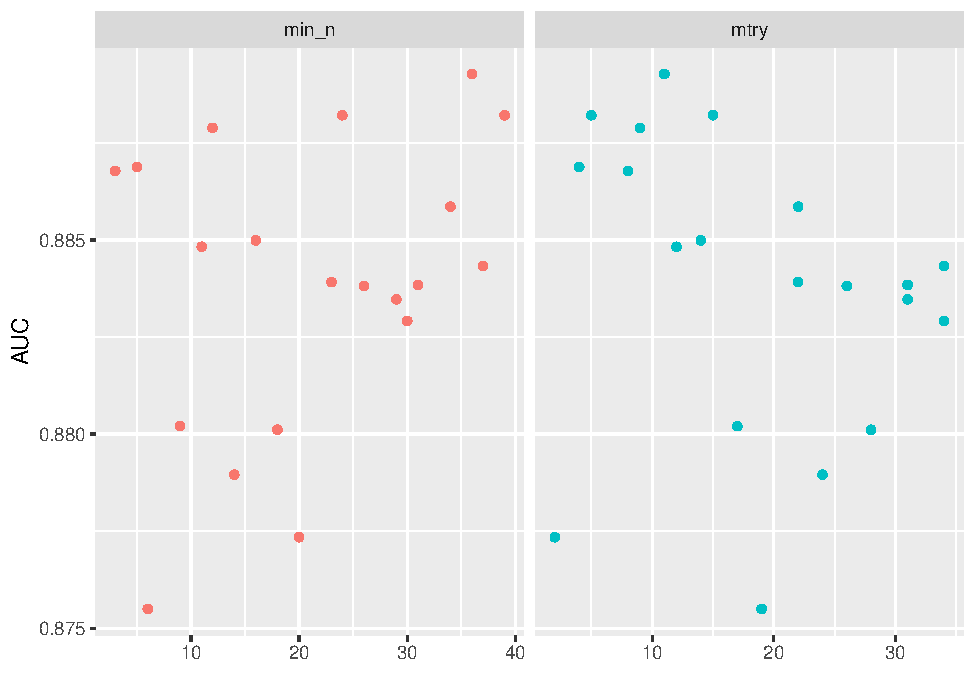
\includegraphics{model_spec_files/figure-latex/unnamed-chunk-11-1.pdf}

\hypertarget{tuning-from-regular-grid}{%
\section{Tuning from regular grid}\label{tuning-from-regular-grid}}

\begin{Shaded}
\begin{Highlighting}[]
\CommentTok{# Regular grid search from previous plot}

\NormalTok{rf_grid <-}\StringTok{ }\KeywordTok{grid_regular}\NormalTok{(}
  \KeywordTok{mtry}\NormalTok{(}\DataTypeTok{range =} \KeywordTok{c}\NormalTok{(}\DecValTok{6}\NormalTok{, }\DecValTok{15}\NormalTok{)),}
  \KeywordTok{min_n}\NormalTok{(}\DataTypeTok{range =} \KeywordTok{c}\NormalTok{(}\DecValTok{30}\NormalTok{, }\DecValTok{45}\NormalTok{)),}
  \DataTypeTok{levels =} \DecValTok{5}
\NormalTok{)}

\NormalTok{rf_grid}
\end{Highlighting}
\end{Shaded}

\hypertarget{a-tibble-25-x-2}{%
\section{A tibble: 25 x 2}\label{a-tibble-25-x-2}}

\begin{verbatim}
mtry min_n
\end{verbatim}

1 6 30 2 8 30 3 10 30 4 12 30 5 15 30 6 6 33 7 8 33 8 10 33 9 12 33 10
15 33 \# \ldots{} with 15 more rows

\begin{Shaded}
\begin{Highlighting}[]
\CommentTok{#tail(rf_grid)}


\CommentTok{# Tuning over regular grid of hyper parameter value }
\CommentTok{# for finding the best model}



\NormalTok{regular_res <-}\StringTok{ }\KeywordTok{tune_grid}\NormalTok{(}
\NormalTok{  tune_wf,}
  \DataTypeTok{resamples =}\NormalTok{ trees_folds,}
  \DataTypeTok{grid =}\NormalTok{ rf_grid}
\NormalTok{)}

\CommentTok{#regular_res}

\CommentTok{# Plotting the accuracy matrix for combination of tuning parameter}

\NormalTok{regular_res }\OperatorTok
\StringTok{  }\KeywordTok{collect_metrics}\NormalTok{() }\OperatorTok
\StringTok{  }\KeywordTok{filter}\NormalTok{(.metric }\OperatorTok{==}\StringTok{ "roc_auc"}\NormalTok{) }\OperatorTok
\StringTok{  }\KeywordTok{mutate}\NormalTok{(}\DataTypeTok{min_n =} \KeywordTok{factor}\NormalTok{(min_n)) }\OperatorTok
\StringTok{  }\KeywordTok{ggplot}\NormalTok{(}\KeywordTok{aes}\NormalTok{(mtry, mean, }\DataTypeTok{color =}\NormalTok{ min_n)) }\OperatorTok{+}
\StringTok{  }\KeywordTok{geom_line}\NormalTok{(}\DataTypeTok{alpha =} \FloatTok{0.5}\NormalTok{, }\DataTypeTok{size =} \FloatTok{1.5}\NormalTok{) }\OperatorTok{+}
\StringTok{  }\KeywordTok{geom_point}\NormalTok{() }\OperatorTok{+}
\StringTok{  }\KeywordTok{labs}\NormalTok{(}\DataTypeTok{y =} \StringTok{"AUC"}\NormalTok{)}
\end{Highlighting}
\end{Shaded}

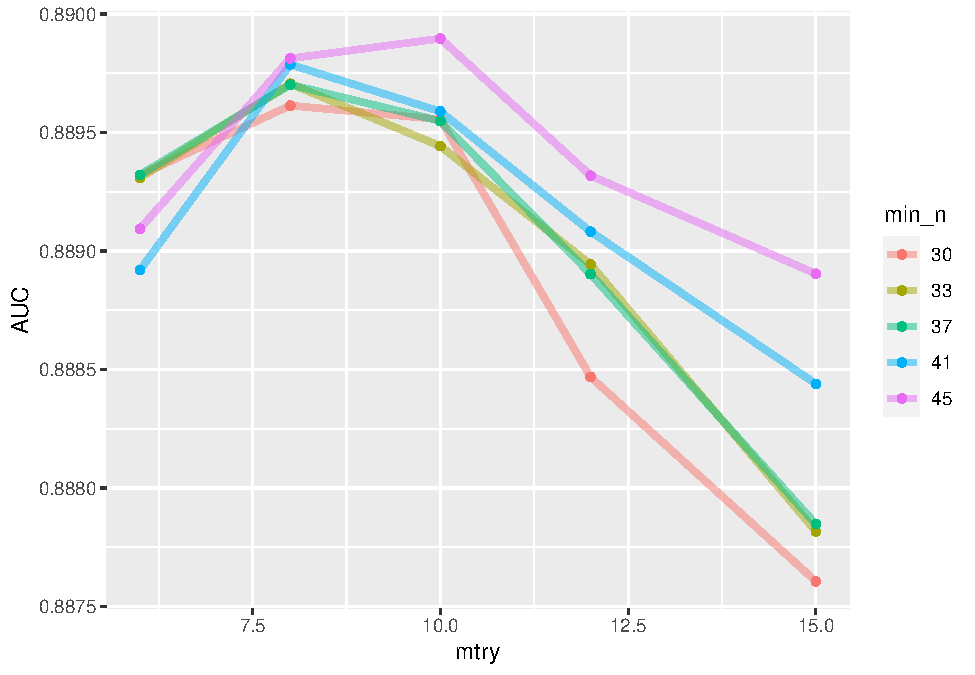
\includegraphics{model_spec_files/figure-latex/unnamed-chunk-12-1.pdf}

\hypertarget{selecting-the-best-model}{%
\section{Selecting the best model}\label{selecting-the-best-model}}

\begin{Shaded}
\begin{Highlighting}[]
\CommentTok{# Choosing best model}


\NormalTok{best_auc <-}\StringTok{ }\KeywordTok{select_best}\NormalTok{(regular_res, }\StringTok{"roc_auc"}\NormalTok{)}

\NormalTok{final_rf <-}\StringTok{ }\KeywordTok{finalize_model}\NormalTok{(}
\NormalTok{  tune_spec,}
\NormalTok{  best_auc}
\NormalTok{)}




\CommentTok{# Variable importance plot}


\NormalTok{tree_fit <-}\StringTok{ }\NormalTok{final_rf }\OperatorTok
\StringTok{  }\KeywordTok{set_engine}\NormalTok{(}\StringTok{"ranger"}\NormalTok{, }\DataTypeTok{importance =} \StringTok{"permutation"}\NormalTok{) }\OperatorTok
\StringTok{  }\KeywordTok{fit}\NormalTok{(over_50k }\OperatorTok{~}\StringTok{ }\NormalTok{.,}
      \DataTypeTok{data =} \KeywordTok{juice}\NormalTok{(tree_prep) }\OperatorTok\StringTok{ }\KeywordTok{select}\NormalTok{(}\OperatorTok{-}\NormalTok{id)}
\NormalTok{  )}


\CommentTok{# Creating variable importance plot of top 10 feature}

\NormalTok{tree_fit }\OperatorTok
\StringTok{  }\KeywordTok{vip}\NormalTok{(}\DataTypeTok{geom =} \StringTok{"point"}\NormalTok{, }\DataTypeTok{num_features =} \DecValTok{10}\NormalTok{)}
\end{Highlighting}
\end{Shaded}

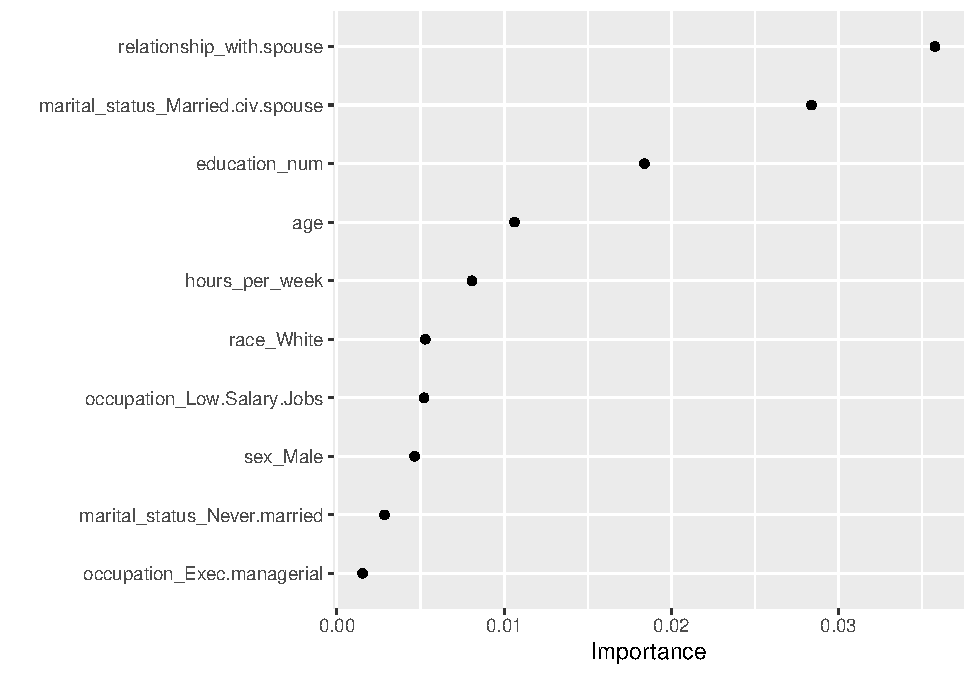
\includegraphics{model_spec_files/figure-latex/unnamed-chunk-13-1.pdf}

\begin{Shaded}
\begin{Highlighting}[]
\NormalTok{final_wf <-}\StringTok{ }\KeywordTok{workflow}\NormalTok{() }\OperatorTok
\StringTok{  }\KeywordTok{add_recipe}\NormalTok{(tree_rec) }\OperatorTok
\StringTok{  }\KeywordTok{add_model}\NormalTok{(final_rf)}

\NormalTok{final_res <-}\StringTok{ }\NormalTok{final_wf }\OperatorTok
\StringTok{  }\KeywordTok{last_fit}\NormalTok{(train_test_split)}


\CommentTok{# Final accuracy from validation set}

\NormalTok{final_res }\OperatorTok
\StringTok{  }\KeywordTok{collect_metrics}\NormalTok{()}
\end{Highlighting}
\end{Shaded}

\hypertarget{a-tibble-2-x-3}{%
\section{A tibble: 2 x 3}\label{a-tibble-2-x-3}}

.metric .estimator .estimate 1 accuracy binary 0.870 2 roc\_auc binary
0.884

\begin{Shaded}
\begin{Highlighting}[]
\CommentTok{# Prediction on full data using the trained model}

\NormalTok{prediction_df <-}\StringTok{ }\NormalTok{df_cleaned }\OperatorTok\StringTok{ }
\StringTok{  }\KeywordTok{mutate}\NormalTok{(}\DataTypeTok{prediction =}\NormalTok{ tree_fit }\OperatorTok\StringTok{ }\KeywordTok{predict}\NormalTok{(}\DataTypeTok{new_data =} \KeywordTok{bake}\NormalTok{(}\DataTypeTok{object =}\NormalTok{ tree_prep, }\DataTypeTok{new_data =}\NormalTok{ df_cleaned)) }\OperatorTok\StringTok{ }\KeywordTok{unlist}\NormalTok{()) }\OperatorTok\StringTok{ }
\StringTok{  }\KeywordTok{select}\NormalTok{(id, prediction, over_50k)}

\KeywordTok{head}\NormalTok{(prediction_df)}
\end{Highlighting}
\end{Shaded}

\hypertarget{a-tibble-6-x-3}{%
\section{A tibble: 6 x 3}\label{a-tibble-6-x-3}}

\begin{verbatim}
 id prediction over_50k
\end{verbatim}

\\
1 12106 \textless{}=50K \textless{}=50K\\
2 28951 \textless{}=50K \textless{}=50K\\
3 24570 \textless{}=50K \textgreater{}50K\\
4 16358 \textless{}=50K \textless{}=50K\\
5 9375 \textless{}=50K \textless{}=50K\\
6 10738 \textgreater{}50K \textgreater{}50K

\begin{Shaded}
\begin{Highlighting}[]
\CommentTok{# Confusion matrix on full data}

\CommentTok{#tabyl(prediction_df, prediction, over_50k)}
\end{Highlighting}
\end{Shaded}

\hypertarget{saving-the-prediction-dataset}{%
\section{Saving the prediction
dataset}\label{saving-the-prediction-dataset}}

\begin{Shaded}
\begin{Highlighting}[]
\CommentTok{# Saving the predictions}

\NormalTok{prediction_df }\OperatorTok\StringTok{ }
\StringTok{  }\KeywordTok{select}\NormalTok{(}\OperatorTok{-}\NormalTok{over_50k) }\OperatorTok\StringTok{ }
\StringTok{  }\KeywordTok{write_csv}\NormalTok{(}\StringTok{"prediction-dataset.csv"}\NormalTok{)}
\end{Highlighting}
\end{Shaded}

End of analysis

\end{document}
